% Created by tikzDevice version 0.10.1 on 2016-04-29 09:35:49
% !TEX encoding = UTF-8 Unicode
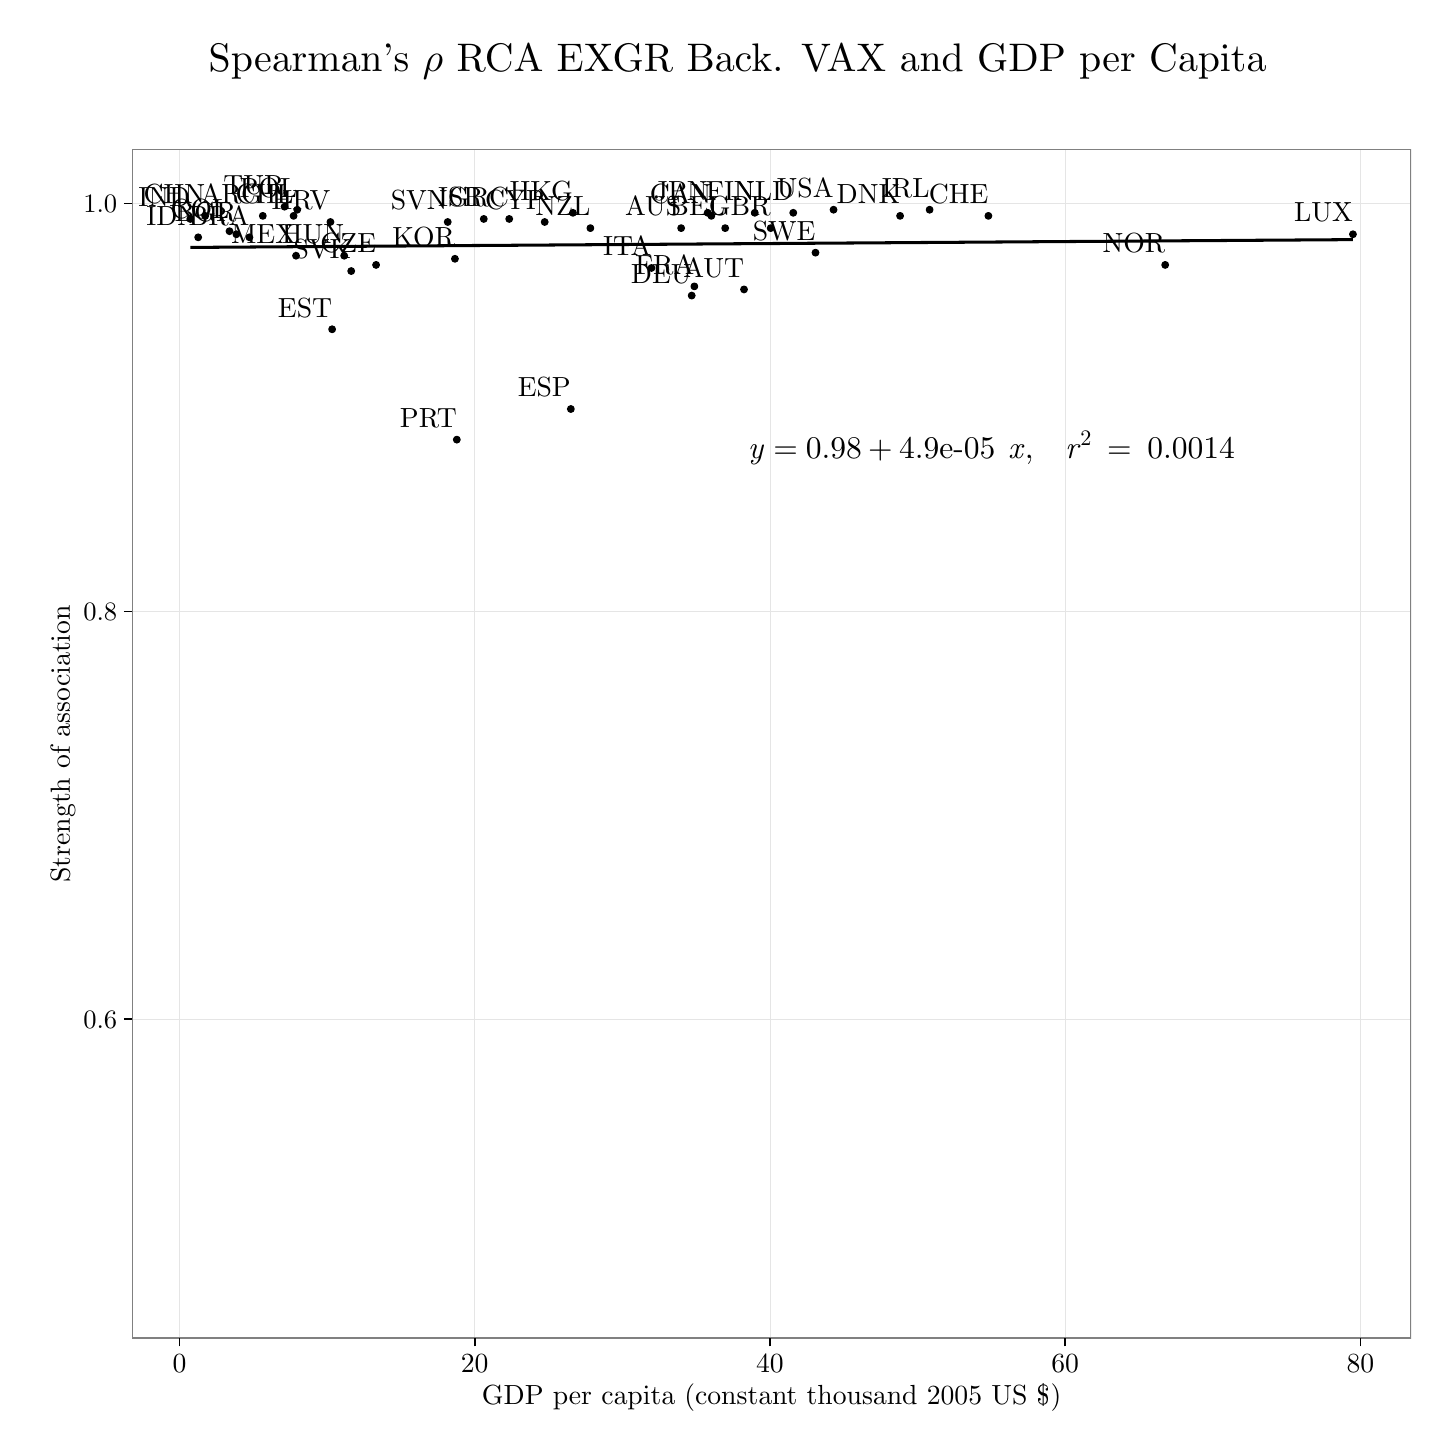
\begin{tikzpicture}[x=1pt,y=1pt]
\definecolor{fillColor}{RGB}{255,255,255}
\path[use as bounding box,fill=fillColor,fill opacity=0.00] (0,0) rectangle (505.89,505.89);
\begin{scope}
\path[clip] (  0.00,  0.00) rectangle (505.89,505.89);
\definecolor{drawColor}{RGB}{255,255,255}
\definecolor{fillColor}{RGB}{255,255,255}

\path[draw=drawColor,line width= 0.6pt,line join=round,line cap=round,fill=fillColor] (  0.00,  0.00) rectangle (505.89,505.89);
\end{scope}
\begin{scope}
\path[clip] ( 37.75, 32.37) rectangle (499.89,461.83);
\definecolor{fillColor}{RGB}{255,255,255}

\path[fill=fillColor] ( 37.75, 32.37) rectangle (499.89,461.83);
\definecolor{drawColor}{gray}{0.90}

\path[draw=drawColor,line width= 0.2pt,line join=round] ( 37.75,147.66) --
	(499.89,147.66);

\path[draw=drawColor,line width= 0.2pt,line join=round] ( 37.75,294.98) --
	(499.89,294.98);

\path[draw=drawColor,line width= 0.2pt,line join=round] ( 37.75,442.31) --
	(499.89,442.31);

\path[draw=drawColor,line width= 0.2pt,line join=round] ( 54.87, 32.37) --
	( 54.87,461.83);

\path[draw=drawColor,line width= 0.2pt,line join=round] (161.55, 32.37) --
	(161.55,461.83);

\path[draw=drawColor,line width= 0.2pt,line join=round] (268.23, 32.37) --
	(268.23,461.83);

\path[draw=drawColor,line width= 0.2pt,line join=round] (374.90, 32.37) --
	(374.90,461.83);

\path[draw=drawColor,line width= 0.2pt,line join=round] (481.58, 32.37) --
	(481.58,461.83);
\definecolor{drawColor}{RGB}{0,0,0}
\definecolor{fillColor}{RGB}{0,0,0}

\path[draw=drawColor,line width= 0.4pt,line join=round,line cap=round,fill=fillColor] ( 84.96,437.88) circle (  1.21);

\path[draw=drawColor,line width= 0.4pt,line join=round,line cap=round,fill=fillColor] (236.13,433.45) circle (  1.21);

\path[draw=drawColor,line width= 0.4pt,line join=round,line cap=round,fill=fillColor] (258.85,411.30) circle (  1.21);

\path[draw=drawColor,line width= 0.4pt,line join=round,line cap=round,fill=fillColor] (252.05,433.45) circle (  1.21);

\path[draw=drawColor,line width= 0.4pt,line join=round,line cap=round,fill=fillColor] ( 75.42,431.23) circle (  1.21);

\path[draw=drawColor,line width= 0.4pt,line join=round,line cap=round,fill=fillColor] ( 80.12,430.13) circle (  1.21);

\path[draw=drawColor,line width= 0.4pt,line join=round,line cap=round,fill=fillColor] (247.04,437.88) circle (  1.21);

\path[draw=drawColor,line width= 0.4pt,line join=round,line cap=round,fill=fillColor] (347.15,437.88) circle (  1.21);

\path[draw=drawColor,line width= 0.4pt,line join=round,line cap=round,fill=fillColor] ( 96.09,437.88) circle (  1.21);

\path[draw=drawColor,line width= 0.4pt,line join=round,line cap=round,fill=fillColor] ( 64.15,437.88) circle (  1.21);

\path[draw=drawColor,line width= 0.4pt,line join=round,line cap=round,fill=fillColor] ( 72.93,432.34) circle (  1.21);

\path[draw=drawColor,line width= 0.4pt,line join=round,line cap=round,fill=fillColor] (186.82,435.67) circle (  1.21);

\path[draw=drawColor,line width= 0.4pt,line join=round,line cap=round,fill=fillColor] (125.90,420.16) circle (  1.21);

\path[draw=drawColor,line width= 0.4pt,line join=round,line cap=round,fill=fillColor] (239.94,409.08) circle (  1.21);

\path[draw=drawColor,line width= 0.4pt,line join=round,line cap=round,fill=fillColor] (315.25,437.88) circle (  1.21);

\path[draw=drawColor,line width= 0.4pt,line join=round,line cap=round,fill=fillColor] (196.27,368.09) circle (  1.21);

\path[draw=drawColor,line width= 0.4pt,line join=round,line cap=round,fill=fillColor] (110.01,396.90) circle (  1.21);

\path[draw=drawColor,line width= 0.4pt,line join=round,line cap=round,fill=fillColor] (262.73,438.99) circle (  1.21);

\path[draw=drawColor,line width= 0.4pt,line join=round,line cap=round,fill=fillColor] (240.91,412.40) circle (  1.21);

\path[draw=drawColor,line width= 0.4pt,line join=round,line cap=round,fill=fillColor] (268.48,433.45) circle (  1.21);

\path[draw=drawColor,line width= 0.4pt,line join=round,line cap=round,fill=fillColor] (174.01,436.77) circle (  1.21);

\path[draw=drawColor,line width= 0.4pt,line join=round,line cap=round,fill=fillColor] (197.02,438.99) circle (  1.21);

\path[draw=drawColor,line width= 0.4pt,line join=round,line cap=round,fill=fillColor] (109.40,435.67) circle (  1.21);

\path[draw=drawColor,line width= 0.4pt,line join=round,line cap=round,fill=fillColor] (114.37,423.48) circle (  1.21);

\path[draw=drawColor,line width= 0.4pt,line join=round,line cap=round,fill=fillColor] ( 61.61,430.13) circle (  1.21);

\path[draw=drawColor,line width= 0.4pt,line join=round,line cap=round,fill=fillColor] ( 58.76,436.77) circle (  1.21);

\path[draw=drawColor,line width= 0.4pt,line join=round,line cap=round,fill=fillColor] (325.91,440.10) circle (  1.21);

\path[draw=drawColor,line width= 0.4pt,line join=round,line cap=round,fill=fillColor] (164.81,436.77) circle (  1.21);

\path[draw=drawColor,line width= 0.4pt,line join=round,line cap=round,fill=fillColor] (225.41,419.05) circle (  1.21);

\path[draw=drawColor,line width= 0.4pt,line join=round,line cap=round,fill=fillColor] (245.72,438.99) circle (  1.21);

\path[draw=drawColor,line width= 0.4pt,line join=round,line cap=round,fill=fillColor] (154.39,422.37) circle (  1.21);

\path[draw=drawColor,line width= 0.4pt,line join=round,line cap=round,fill=fillColor] (478.88,431.23) circle (  1.21);

\path[draw=drawColor,line width= 0.4pt,line join=round,line cap=round,fill=fillColor] ( 96.97,423.48) circle (  1.21);

\path[draw=drawColor,line width= 0.4pt,line join=round,line cap=round,fill=fillColor] (276.64,438.99) circle (  1.21);

\path[draw=drawColor,line width= 0.4pt,line join=round,line cap=round,fill=fillColor] (411.04,420.16) circle (  1.21);

\path[draw=drawColor,line width= 0.4pt,line join=round,line cap=round,fill=fillColor] (203.33,433.45) circle (  1.21);

\path[draw=drawColor,line width= 0.4pt,line join=round,line cap=round,fill=fillColor] ( 97.41,440.10) circle (  1.21);

\path[draw=drawColor,line width= 0.4pt,line join=round,line cap=round,fill=fillColor] (155.07,357.02) circle (  1.21);

\path[draw=drawColor,line width= 0.4pt,line join=round,line cap=round,fill=fillColor] (116.91,417.94) circle (  1.21);

\path[draw=drawColor,line width= 0.4pt,line join=round,line cap=round,fill=fillColor] (151.78,435.67) circle (  1.21);

\path[draw=drawColor,line width= 0.4pt,line join=round,line cap=round,fill=fillColor] (284.68,424.59) circle (  1.21);

\path[draw=drawColor,line width= 0.4pt,line join=round,line cap=round,fill=fillColor] ( 92.83,441.20) circle (  1.21);

\path[draw=drawColor,line width= 0.4pt,line join=round,line cap=round,fill=fillColor] (291.20,440.10) circle (  1.21);

\node[text=drawColor,anchor=base east,inner sep=0pt, outer sep=0pt, scale=  1.0] at ( 84.96,442.32) {ARG};

\node[text=drawColor,anchor=base east,inner sep=0pt, outer sep=0pt, scale=  1.0] at (236.13,437.89) {AUS};

\node[text=drawColor,anchor=base east,inner sep=0pt, outer sep=0pt, scale=  1.0] at (258.85,415.74) {AUT};

\node[text=drawColor,anchor=base east,inner sep=0pt, outer sep=0pt, scale=  1.0] at (252.05,437.89) {BEL};

\node[text=drawColor,anchor=base east,inner sep=0pt, outer sep=0pt, scale=  1.0] at ( 75.42,435.68) {BGR};

\node[text=drawColor,anchor=base east,inner sep=0pt, outer sep=0pt, scale=  1.0] at ( 80.12,434.57) {BRA};

\node[text=drawColor,anchor=base east,inner sep=0pt, outer sep=0pt, scale=  1.0] at (247.04,442.32) {CAN};

\node[text=drawColor,anchor=base east,inner sep=0pt, outer sep=0pt, scale=  1.0] at (347.15,442.32) {CHE};

\node[text=drawColor,anchor=base east,inner sep=0pt, outer sep=0pt, scale=  1.0] at ( 96.09,442.32) {CHL};

\node[text=drawColor,anchor=base east,inner sep=0pt, outer sep=0pt, scale=  1.0] at ( 64.15,442.32) {CHN};

\node[text=drawColor,anchor=base east,inner sep=0pt, outer sep=0pt, scale=  1.0] at ( 72.93,436.78) {COL};

\node[text=drawColor,anchor=base east,inner sep=0pt, outer sep=0pt, scale=  1.0] at (186.82,440.11) {CYP};

\node[text=drawColor,anchor=base east,inner sep=0pt, outer sep=0pt, scale=  1.0] at (125.90,424.60) {CZE};

\node[text=drawColor,anchor=base east,inner sep=0pt, outer sep=0pt, scale=  1.0] at (239.94,413.52) {DEU};

\node[text=drawColor,anchor=base east,inner sep=0pt, outer sep=0pt, scale=  1.0] at (315.25,442.32) {DNK};

\node[text=drawColor,anchor=base east,inner sep=0pt, outer sep=0pt, scale=  1.0] at (196.27,372.54) {ESP};

\node[text=drawColor,anchor=base east,inner sep=0pt, outer sep=0pt, scale=  1.0] at (110.01,401.34) {EST};

\node[text=drawColor,anchor=base east,inner sep=0pt, outer sep=0pt, scale=  1.0] at (262.73,443.43) {FIN};

\node[text=drawColor,anchor=base east,inner sep=0pt, outer sep=0pt, scale=  1.0] at (240.91,416.85) {FRA};

\node[text=drawColor,anchor=base east,inner sep=0pt, outer sep=0pt, scale=  1.0] at (268.48,437.89) {GBR};

\node[text=drawColor,anchor=base east,inner sep=0pt, outer sep=0pt, scale=  1.0] at (174.01,441.22) {GRC};

\node[text=drawColor,anchor=base east,inner sep=0pt, outer sep=0pt, scale=  1.0] at (197.02,443.43) {HKG};

\node[text=drawColor,anchor=base east,inner sep=0pt, outer sep=0pt, scale=  1.0] at (109.40,440.11) {HRV};

\node[text=drawColor,anchor=base east,inner sep=0pt, outer sep=0pt, scale=  1.0] at (114.37,427.92) {HUN};

\node[text=drawColor,anchor=base east,inner sep=0pt, outer sep=0pt, scale=  1.0] at ( 61.61,434.57) {IDN};

\node[text=drawColor,anchor=base east,inner sep=0pt, outer sep=0pt, scale=  1.0] at ( 58.76,441.22) {IND};

\node[text=drawColor,anchor=base east,inner sep=0pt, outer sep=0pt, scale=  1.0] at (325.91,444.54) {IRL};

\node[text=drawColor,anchor=base east,inner sep=0pt, outer sep=0pt, scale=  1.0] at (164.81,441.22) {ISR};

\node[text=drawColor,anchor=base east,inner sep=0pt, outer sep=0pt, scale=  1.0] at (225.41,423.49) {ITA};

\node[text=drawColor,anchor=base east,inner sep=0pt, outer sep=0pt, scale=  1.0] at (245.72,443.43) {JPN};

\node[text=drawColor,anchor=base east,inner sep=0pt, outer sep=0pt, scale=  1.0] at (154.39,426.82) {KOR};

\node[text=drawColor,anchor=base east,inner sep=0pt, outer sep=0pt, scale=  1.0] at (478.88,435.68) {LUX};

\node[text=drawColor,anchor=base east,inner sep=0pt, outer sep=0pt, scale=  1.0] at ( 96.97,427.92) {MEX};

\node[text=drawColor,anchor=base east,inner sep=0pt, outer sep=0pt, scale=  1.0] at (276.64,443.43) {NLD};

\node[text=drawColor,anchor=base east,inner sep=0pt, outer sep=0pt, scale=  1.0] at (411.04,424.60) {NOR};

\node[text=drawColor,anchor=base east,inner sep=0pt, outer sep=0pt, scale=  1.0] at (203.33,437.89) {NZL};

\node[text=drawColor,anchor=base east,inner sep=0pt, outer sep=0pt, scale=  1.0] at ( 97.41,444.54) {POL};

\node[text=drawColor,anchor=base east,inner sep=0pt, outer sep=0pt, scale=  1.0] at (155.07,361.46) {PRT};

\node[text=drawColor,anchor=base east,inner sep=0pt, outer sep=0pt, scale=  1.0] at (116.91,422.38) {SVK};

\node[text=drawColor,anchor=base east,inner sep=0pt, outer sep=0pt, scale=  1.0] at (151.78,440.11) {SVN};

\node[text=drawColor,anchor=base east,inner sep=0pt, outer sep=0pt, scale=  1.0] at (284.68,429.03) {SWE};

\node[text=drawColor,anchor=base east,inner sep=0pt, outer sep=0pt, scale=  1.0] at ( 92.83,445.65) {TUR};

\node[text=drawColor,anchor=base east,inner sep=0pt, outer sep=0pt, scale=  1.0] at (291.20,444.54) {USA};

\path[draw=drawColor,line width= 1.1pt,line join=round] ( 58.76,426.48) --
	( 64.08,426.51) --
	( 69.39,426.55) --
	( 74.71,426.59) --
	( 80.03,426.62) --
	( 85.35,426.66) --
	( 90.67,426.69) --
	( 95.98,426.73) --
	(101.30,426.76) --
	(106.62,426.80) --
	(111.94,426.83) --
	(117.26,426.87) --
	(122.57,426.91) --
	(127.89,426.94) --
	(133.21,426.98) --
	(138.53,427.01) --
	(143.85,427.05) --
	(149.16,427.08) --
	(154.48,427.12) --
	(159.80,427.16) --
	(165.12,427.19) --
	(170.44,427.23) --
	(175.75,427.26) --
	(181.07,427.30) --
	(186.39,427.33) --
	(191.71,427.37) --
	(197.03,427.41) --
	(202.34,427.44) --
	(207.66,427.48) --
	(212.98,427.51) --
	(218.30,427.55) --
	(223.62,427.58) --
	(228.94,427.62) --
	(234.25,427.65) --
	(239.57,427.69) --
	(244.89,427.73) --
	(250.21,427.76) --
	(255.53,427.80) --
	(260.84,427.83) --
	(266.16,427.87) --
	(271.48,427.90) --
	(276.80,427.94) --
	(282.12,427.98) --
	(287.43,428.01) --
	(292.75,428.05) --
	(298.07,428.08) --
	(303.39,428.12) --
	(308.71,428.15) --
	(314.02,428.19) --
	(319.34,428.23) --
	(324.66,428.26) --
	(329.98,428.30) --
	(335.30,428.33) --
	(340.61,428.37) --
	(345.93,428.40) --
	(351.25,428.44) --
	(356.57,428.47) --
	(361.89,428.51) --
	(367.20,428.55) --
	(372.52,428.58) --
	(377.84,428.62) --
	(383.16,428.65) --
	(388.48,428.69) --
	(393.79,428.72) --
	(399.11,428.76) --
	(404.43,428.80) --
	(409.75,428.83) --
	(415.07,428.87) --
	(420.39,428.90) --
	(425.70,428.94) --
	(431.02,428.97) --
	(436.34,429.01) --
	(441.66,429.05) --
	(446.98,429.08) --
	(452.29,429.12) --
	(457.61,429.15) --
	(462.93,429.19) --
	(468.25,429.22) --
	(473.57,429.26) --
	(478.88,429.30);

\node[text=drawColor,anchor=base west,inner sep=0pt, outer sep=0pt, scale=  1.14] at (260.28,350.14) {\itshape y};

\node[text=drawColor,anchor=base west,inner sep=0pt, outer sep=0pt, scale=  1.14] at (269.44,350.14) {=};

\node[text=drawColor,anchor=base west,inner sep=0pt, outer sep=0pt, scale=  1.14] at (281.18,350.14) {0.98};

\node[text=drawColor,anchor=base west,inner sep=0pt, outer sep=0pt, scale=  1.14] at (303.73,350.14) {+};

\node[text=drawColor,anchor=base west,inner sep=0pt, outer sep=0pt, scale=  1.14] at (314.89,350.14) {4.9e-05};

\node[text=drawColor,anchor=base west,inner sep=0pt, outer sep=0pt, scale=  1.14] at (351.97,350.14) {};

\node[text=drawColor,anchor=base west,inner sep=0pt, outer sep=0pt, scale=  1.14] at (354.29,350.14) {\itshape x};

\node[text=drawColor,anchor=base west,inner sep=0pt, outer sep=0pt, scale=  1.14] at (360.30,350.14) {,};

\node[text=drawColor,anchor=base west,inner sep=0pt, outer sep=0pt, scale=  1.14] at (363.47,350.14) { };

\node[text=drawColor,anchor=base west,inner sep=0pt, outer sep=0pt, scale=  1.14] at (369.15,350.14) { };

\node[text=drawColor,anchor=base west,inner sep=0pt, outer sep=0pt, scale=  1.14] at (374.84,350.14) {\itshape r};

\node[text=drawColor,anchor=base west,inner sep=0pt, outer sep=0pt, scale=  0.80] at (380.37,354.79) {2};

\node[text=drawColor,anchor=base west,inner sep=0pt, outer sep=0pt, scale=  1.14] at (384.36,350.14) { };

\node[text=drawColor,anchor=base west,inner sep=0pt, outer sep=0pt, scale=  1.14] at (390.05,350.14) {=};

\node[text=drawColor,anchor=base west,inner sep=0pt, outer sep=0pt, scale=  1.14] at (398.89,350.14) { };

\node[text=drawColor,anchor=base west,inner sep=0pt, outer sep=0pt, scale=  1.14] at (404.58,350.14) {0.0014};
\definecolor{drawColor}{gray}{0.50}

\path[draw=drawColor,line width= 0.6pt,line join=round,line cap=round] ( 37.75, 32.37) rectangle (499.89,461.83);
\end{scope}
\begin{scope}
\path[clip] (  0.00,  0.00) rectangle (505.89,505.89);
\definecolor{drawColor}{RGB}{0,0,0}

\node[text=drawColor,anchor=base east,inner sep=0pt, outer sep=0pt, scale=  0.96] at ( 32.35,144.35) {0.6};

\node[text=drawColor,anchor=base east,inner sep=0pt, outer sep=0pt, scale=  0.96] at ( 32.35,291.68) {0.8};

\node[text=drawColor,anchor=base east,inner sep=0pt, outer sep=0pt, scale=  0.96] at ( 32.35,439.01) {1.0};
\end{scope}
\begin{scope}
\path[clip] (  0.00,  0.00) rectangle (505.89,505.89);
\definecolor{drawColor}{RGB}{0,0,0}

\path[draw=drawColor,line width= 0.6pt,line join=round] ( 34.75,147.66) --
	( 37.75,147.66);

\path[draw=drawColor,line width= 0.6pt,line join=round] ( 34.75,294.98) --
	( 37.75,294.98);

\path[draw=drawColor,line width= 0.6pt,line join=round] ( 34.75,442.31) --
	( 37.75,442.31);
\end{scope}
\begin{scope}
\path[clip] (  0.00,  0.00) rectangle (505.89,505.89);
\definecolor{drawColor}{RGB}{0,0,0}

\path[draw=drawColor,line width= 0.6pt,line join=round] ( 54.87, 29.37) --
	( 54.87, 32.37);

\path[draw=drawColor,line width= 0.6pt,line join=round] (161.55, 29.37) --
	(161.55, 32.37);

\path[draw=drawColor,line width= 0.6pt,line join=round] (268.23, 29.37) --
	(268.23, 32.37);

\path[draw=drawColor,line width= 0.6pt,line join=round] (374.90, 29.37) --
	(374.90, 32.37);

\path[draw=drawColor,line width= 0.6pt,line join=round] (481.58, 29.37) --
	(481.58, 32.37);
\end{scope}
\begin{scope}
\path[clip] (  0.00,  0.00) rectangle (505.89,505.89);
\definecolor{drawColor}{RGB}{0,0,0}

\node[text=drawColor,anchor=base,inner sep=0pt, outer sep=0pt, scale=  1.00] at ( 54.87, 20.09) {0};

\node[text=drawColor,anchor=base,inner sep=0pt, outer sep=0pt, scale=  1.00] at (161.55, 20.09) {20};

\node[text=drawColor,anchor=base,inner sep=0pt, outer sep=0pt, scale=  1.00] at (268.23, 20.09) {40};

\node[text=drawColor,anchor=base,inner sep=0pt, outer sep=0pt, scale=  1.00] at (374.90, 20.09) {60};

\node[text=drawColor,anchor=base,inner sep=0pt, outer sep=0pt, scale=  1.00] at (481.58, 20.09) {80};
\end{scope}
\begin{scope}
\path[clip] (  0.00,  0.00) rectangle (505.89,505.89);
\definecolor{drawColor}{RGB}{0,0,0}

\node[text=drawColor,anchor=base,inner sep=0pt, outer sep=0pt, scale=  1.00] at (268.82,  8.40) {GDP per capita (constant thousand 2005 US \$)};
\end{scope}
\begin{scope}
\path[clip] (  0.00,  0.00) rectangle (505.89,505.89);
\definecolor{drawColor}{RGB}{0,0,0}

\node[text=drawColor,rotate= 90.00,anchor=base,inner sep=0pt, outer sep=0pt, scale=  1.00] at ( 15.29,247.10) {Strength of association};
\end{scope}
\begin{scope}
\path[clip] (  0.00,  0.00) rectangle (505.89,505.89);
\definecolor{drawColor}{RGB}{0,0,0}

\node[text=drawColor,anchor=base west,inner sep=0pt, outer sep=0pt, scale=  1.44] at ( 65.41,489.97) {Spearman's $\rho$ RCA EXGR Back. VAX and GDP per Capita};
\end{scope}
\end{tikzpicture}
